
\chapter{Fundamentação Teórica}
\label{cap-fundamentacao}


Opa! Testando arquivo de fundamentação.


\section{Big Data}
\subsection{Frameworks e ferramentas de gerenciamento de aplicações}
\subsubsection{Conteinerização}
Docker...


\subsubsection{Gerenciamento de Cluster}
Kubernetes...



\section{Paradigmas de Desenvolvimento}


\section{Paradigma Orientado a Notificações (PON)}


O PON é um paradigma emergente que teve origem em uma solução de controle discreto para a indústria de manufatura \citep{simaostadzisz2008patentepon}, que posteriormente evoluiu para uma solução geral de controle discreto, uma solução alternativa de inferência e até mesmo um paradigma computacional \citep{simao2012noppicomparison}. 
Como principal diferencial, o PON possui dois grupos de entidades de processamento distintas, a saber: entidades de execução de fatos e entidades lógico-causais, que colaboram por meio de notificações pontuais e precisas, conforme representado na Fig. \ref{fig:examplerule}.

As entidades de execução de fatos lidam com elementos PON e com a execução de procedimentos/ações que alteram seus estados, enquanto as entidades lógico-causais decidem quais ações devem ser executadas. Por sua vez, as entidades de execução de fatos são representadas por Elementos da Base de Fatos (do inglês Fact Base Elements -- FBEs) com seus \textit{Attributes} (Atributos) e \textit{Methods} (Métodos). As entidades lógico-causais são representadas por elementos \textit{Rules} \textit{Regras} com suas \textit{Condition-Premises} (\textit{Condições-Premissas}) e \textit{Actions-Instigations} (\textit{Ações-Instigações}) \citep{linhares2020noca, ronszcka2017noplanguagecompiler}. 
Ainda assim, os \textit{FBEs} e as \textit{Rules}, com seus constituintes, podem ser e geralmente são representados de forma declarativa \citep{neves2021application}.


\begin{figure}[!ht]
\centering
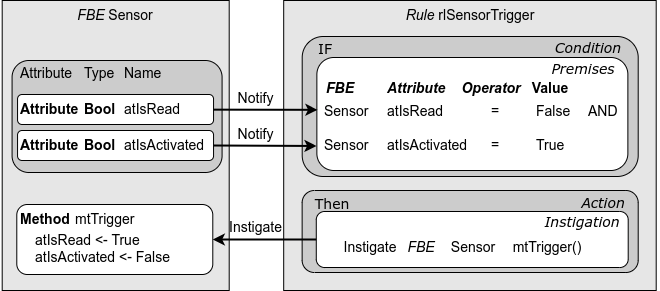
\includegraphics[width=0.8\linewidth]{figuras/example-rule.png}
\caption{Exemplo de instâncias de um Sensor FBE e a Regra rlTriggerSensor com suas partes constituintes para uma aplicação de sensor 
%\cite{neves2021application}.
}
\label{fig:examplerule}
\end{figure}

A Fig. \ref{fig:examplerule} apresenta um exemplo das entidades PON para uma determinada aplicação de sensor. 
O \textit{FBE} denominado Sensor, de certa forma semelhante a uma instância de uma classe no Paradigma Orientado a Objetos (OOP), representa uma espécie de objeto notificador composto por dois \textit{Attributes} booleanos, atIsRead e atIsActivated, e um \textit{Method} denominado mtTrigger que define os valores de atIsRead como verdadeiro e atIsActivated como falso. 
Por sua vez, a \textit{Rule} notificável associada rlSensorTrigger compreende uma \textit{Condition} relacionada a \textit{Premises} e uma \textit{Action} relacionada a uma \textit{Instigation}. Quando ambas as \textit{Premises} da \textit{Condition} são verdadeiras após notificações dos \textit{Attributes} pertinentes, ela aciona a \textit{Rule} rlSensorTrigger, o que faz com que a \textit{Instigation} da \textit{Action} inicie o \textit{Method} mtTrigger a partir do Sensor \textit{FBE}.
Como o exemplo sugere, os componentes \textit{FBE} e \textit{Rule} colaboram por meio de notificações precisas. 


O estado da arte do PON, denominada Linguagem do Paradigma Orientado a Notificações (do inglês Notification-Oriented Paradigm Language -- NOPL), combina uma linguagem de programação e um sistema de compilação para alvos específicos. 
Apesar de apresentar excelente desempenho, o NOPL ainda não foi aplicado a projetos de grande porte ou de nível industrial. Por enquanto, ela é usada para demonstrar as propriedades do PON em aplicações acadêmicas e de benchmark \citep{Babu2022masters, fabro2021nopl}. 
Alternativamente, o estado da arte do PON é a chamada NOP C++ Framework 4.0/4.5 para projetos de grande porte ou industriais. 
Essa estrutura é uma evolução das anteriores e atingiu maturidade para ser aplicada de forma mais ampla. Por ser uma estrutura orientada a notificações sobre C++, alterando a forma usual como o C++ opera, ela é naturalmente menos performática do que a tecnologia NOPL, bastante prototípica, com linguagem e compiladores dedicados. No entanto, essa estrutura ainda é performática e estável para aplicações PON reais \citep{Babu2022masters, fabro2021nopl, pordeus2017masterssimulacao}.


Considerando o exemplo da Fig. \ref{fig:examplerule}, o Algoritmo \ref{alg:lingponstructure} apresenta o código correspondente para o NOPL, e o Algoritmo \ref{alg:frameworkc++} apresenta o código correspondente utilizando o NOP Framework C++ 4.0.
Mais detalhes sobre o NOPL e o NOP Framework C++ podem ser encontrados em \citep{ronszcka2017nopframework2, Negrini2019nopl, fabro2021nopl}.
Na verdade, a estrutura está na fase final do processo de patente e, no momento, não está disponível para a comunidade. No entanto, sua estrutura e detalhes são amplamente divulgados na academia \citep{ronszcka2017nopframework2, ronszcka2015noprete, Babu2022masters}, incluindo os trabalhos citados nesta seção.


\begin{algorithm}[H]
\caption{Exemplo de instruções NOPL para um do FBE Sensor e \textit{Rule} rlTriggerSensor é apresentado na Fig. \ref{fig:examplerule}}
\label{alg:lingponstructure}
\begin{algorithmic}[1]
\STATE \textbf{fbe} Sensor \\
\STATE \hspace{0.1cm} \textbf{private boolean} atIsRead = false \\
\STATE \hspace{0.1cm} \textbf{private boolean} atIsActivated = false \\

\STATE \hspace{0.1cm} \textbf{private method} mtTrigger \\
\STATE \hspace{0.2cm} \textbf{assignment} \\
\STATE \hspace{0.3cm} this.atIsRead = true \\
\STATE \hspace{0.3cm} this.atIsActivated = false \\
\STATE \hspace{0.2cm} \textbf{end\_assignment} \\
\STATE \hspace{0.1cm} \textbf{end\_method} \\

\STATE \hspace{0.1cm} \textbf{rule} rlSensorTrigger \\
\STATE \hspace{0.2cm} \textbf{condition} \\
\STATE \hspace{0.3cm} \textbf{subcondition} \\
\STATE \hspace{0.4cm} \textbf{premise} prIsReadFalse \\
\STATE \hspace{0.5cm} this.atIsRead == false \\
\STATE \hspace{0.4cm} \textbf{end\_premise} \\
\STATE \hspace{0.4cm} \textbf{and} \\
\STATE \hspace{0.4cm} \textbf{premise} prIsActivated \\
\STATE \hspace{0.5cm} this.atIsActivated == true \\
\STATE \hspace{0.4cm} \textbf{end\_premise} \\
\STATE \hspace{0.3cm} \textbf{end\_subcondition} \\
\STATE \hspace{0.2cm} \textbf{end\_condition} \\

\STATE \hspace{0.2cm} \textbf{action sequential} \\
\STATE \hspace{0.3cm} \textbf{instigation sequential} \\
\STATE \hspace{0.4cm} \textbf{call} this.mtTrigger(); \\
\STATE \hspace{0.3cm} \textbf{end\_instigation} \\
\STATE \hspace{0.1cm} \textbf{end\_action} \\
\STATE \hspace{0.cm} \textbf{end\_rule} \\
\STATE\textbf{end\_fbe}

\end{algorithmic}
\end{algorithm}



\begin{algorithm*}
\caption{Exemplo de instruções usando NOP Framework C++ para o \textit{FBE} Sensor e \textit{Rule} rlTriggerSensor presented in Fig. \ref{fig:examplerule}}
  \label{alg:frameworkc++}
  \begin{algorithmic}[1]
\STATE /* Include the NOP Framework C++ 4.0 */ 
\STATE \#\textbf{include} ``libnop\//framework.h''

\STATE \texttt{\\}
\STATE /* Create the class Sensor */ \\
\STATE \textbf{class} Sensor \\ 
\STATE \{ \\
\STATE \hspace{0.cm} \textbf{public}: \\
\STATE \texttt{\\}
\STATE \hspace{0.1cm} /* Create the \textit{Attribute} atIsRead */ \\
\STATE \hspace{0.1cm} \textbf{NOP::SharedAttribute}$<$bool$>$ atIsRead \\
\STATE \hspace{0.1cm} \{ \textbf{NOP::BuildAttribute}$<$bool$>$(false) \}; \\
\STATE \texttt{\\}
\STATE \hspace{0.1cm} /* Create the \textit{Attribute} atIsActivated */ \\
\STATE \hspace{0.1cm} \textbf{NOP::SharedAttribute}$<$bool$>$ atIsActivated \\ 
\STATE \hspace{0.1cm} \{ \textbf{NOP::BuildAttribute}$<$bool$>$(false) \}; \\

\STATE \texttt{\\}

\STATE \hspace{0.1cm} /* Create the \textit{Premise} prIsRead */ \\
\STATE \hspace{0.1cm} \textbf{NOP::SharedPremise} prIsRead \\
\STATE \hspace{0.1cm} \{ \textbf{NOP::BuildPremise}(this.atIsRead, false, \textbf{NOP::Equal()}) \}; \\

\STATE \texttt{\\}

\STATE \hspace{0.1cm} /* Create the \textit{Premise} prIsActivated */ \\
\STATE \hspace{0.1cm} \textbf{NOP::SharedPremise} prIsActivated \\
\STATE \hspace{0.1cm} \{ \textbf{NOP::BuildPremise}(this.atIsActivated, true, \textbf{NOP::Equal()}) \}; \\

\STATE \texttt{\\}

\STATE \hspace{0.1cm} /* Create the \textit{Condition} cnRlSensorTrigger */ \\
\STATE \hspace{0.1cm} \textbf{NOP::SharedCondition} cnRlSensorTrigger = \\
\STATE \hspace{0.1cm}  \textbf{NOP::BuildCondition}$<$\textbf{NOP::Conjunction}$>$(prIsRead, prIsActivated); \\

\STATE \texttt{\\}

\STATE \hspace{0.1cm} /* Create the \textit{Method} mtTrigger */ \\
\STATE \hspace{0.1cm} \textbf{NOP::Method} mtTrigger\{ \\
\STATE \hspace{0.2cm} this.AtIsRead = true; \\
\STATE \hspace{0.2cm} this.atIsActivated = false; \\
\STATE \hspace{0.1cm} \}; \\

\STATE \texttt{\\}

\STATE \hspace{0.1cm} /* Create the \textit{Instigation} inMtTrigger */ \\
\STATE \hspace{0.1cm} \textbf{NOP::SharedInstigation} inMtTrigger = \\
\STATE \hspace{0.1cm} \textbf{NOP::BuildInstigation}(mtTrigger); \\

\STATE \texttt{\\}

\STATE \hspace{0.1cm} /* Create the \textit{Action} acMtTrigger */ \\
\STATE \hspace{0.1cm} \textbf{NOP::SharedAction} acMtTrigger = \\
\STATE \hspace{0.1cm} \textbf{NOP::BuildAction}(inMtTrigger); \\

\STATE \texttt{\\}

\STATE \hspace{0.1cm} /* Create the \textit{Rule} rlSensorTrigger */ \\
\STATE \hspace{0.1cm} \textbf{NOP::SharedRule} rlSensorTrigger = \\
\STATE \hspace{0.1cm} \textbf{NOP::BuildRule}(cnRlSensorTrigger, acMtTrigger); \\

\STATE \texttt{\\}

\STATE /* End class */ \\
\STATE \};  \\

  \end{algorithmic}
\end{algorithm*}


\begin{figure*}[!hb]
\centering
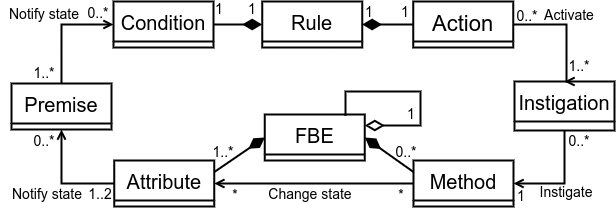
\includegraphics[width=0.99\linewidth]{figuras/original-nop-chain.png}
\caption{Cadeia de inferência PON %\cite{neves2021application}
}
\label{fig:nopmetamodel}
\end{figure*}




Na verdade, o mecanismo central do paradigma é a chamada Cadeia de Inferência PON \citep{peters2012new}, modelada na Fig. \ref{fig:nopmetamodel} e exemplificada na Fig. \ref{fig:notificationflows}.
Cada entidade PON pode enviar e/ou receber notificações precisas e pertinentes, permitindo assim a avaliação de estados apenas quando uma notificação chega.
Esse comportamento colaborativo orientado a notificações oferece uma nova forma de desenvolver e executar aplicativos de software (e até mesmo de hardware) com base em pequenas entidades reativas notificáveis. \citep{linhares2020noca, simao2012noppicomparison}.





\subsection{Cadeia de Inferêcia PON}
\label{sec:nopchain}


Os itens a seguir explicam as entidades NOP de acordo com a cadeia de inferência, levando em consideração a Fig. \ref{fig:nopmetamodel} e a Fig. \ref{fig:notificationflows}:

\begin{itemize}
    \item \textit{Fact Base Element} (\textit{FBE}): Entidade (por exemplo, uma instância de um tipo ou classe) que contém os \textit{Atributes} do notificador e os \textit{Methods} instigadores.
    
    \item \textit{Attribute}: Entidade responsável por armazenar um valor que representa os estados das propriedades de um \textit{FBE} e que pode notificar com precisão as \textit{Premises} relacionadas quando seu valor muda.
    
    \item \textit{Premise}: Entidade que, após ser notificada por um \textit{Attribute}, compara esse \textit{Attribute} com outro \textit{Attribute} ou com uma constante por meio de um operador lógico-relacional (por exemplo, $=$, $\neq$, $>$, $<$) e, subsequentemente, notifica a \textit{Condition} relacionada quando seu estado lógico se altera.
    
    \item \textit{Condition}: Entidade que agrupa uma ou mais \textit{Premises} e, quando notificada por qualquer uma delas, realiza uma operação lógica (por exemplo, conjunção ou disjunção) sobre seus estados e notifica sua \textit{Rule} correspondente se seu valor lógico mudar. 
    
    \item \textit{Rule}: Entidade com uma \textit{Condition} e uma \textit{Action} que determina a execução de sua \textit{Action} quando sua \textit{Condition} é aprovada (por exemplo, seu estado lógico é verdadeiro).
    \item \textit{Action}: Entidade que, quando instigada por sua \textit{Rule}, ativa suas \textit{Instigations} para execução, parametrizando-as adequadamente, se necessário.
    
    \item \textit{Instigation}: Entidade relacionada a uma ou mais \textit{Actions} que, quando instigada por uma \textit{Action}, instiga um conjunto de entidades \textit{Method} a serem executadas, parametrizando-as adequadamente, se necessário.
    
    \item \textit{Methos}: Entidade que, quando instigada por uma \textit{Instigation}, executa uma função ou serviço de um \textit{FBE} e, portanto, pode alterar os estados de \textit{Attributes}, alimentando assim um ciclo de inferência de notificação.
\end{itemize}



\begin{figure*}[tb]
\centering
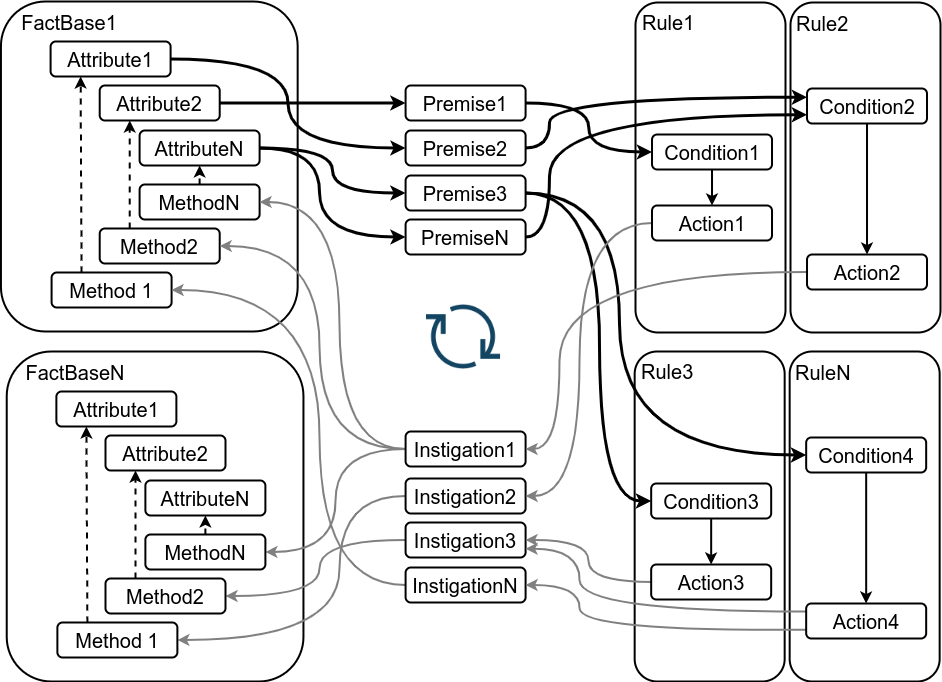
\includegraphics[width=0.99\linewidth]{figuras/notification-flows.png}
\caption{Fluxos de notificação 
%\cite{linhares2020noca}
\label{fig:notificationflows}}
\label{fig:notificationflows}
\end{figure*}


A organização PON reduz ou até mesmo elimina algumas das questões relacionadas aos paradigmas clássicos de desenvolvimento, como o Paradigma Imperativo (IP) e o Paradigma Declarativo (DP), que, respectivamente — e de forma notável —, incluem a Programação Orientada a Objetos (OOP) e os Sistemas Baseados em Regras (RBS) \citep{ronszcka2017nopframework2, linhares2020noca}. 
Exemplos dessas questões são o acoplamento frequentemente forte entre partes do código e as redundâncias estruturais e temporais relacionadas ao processamento de avaliação lógico-causal \citep{ronszcka2017nopframework2}.

As redundâncias estruturais ocorrem quando uma determinada avaliação lógica e/ou causal é repetida desnecessariamente em outra parte do código. 
Por sua vez, as redundâncias temporais ocorrem quando uma determinada avaliação lógica e/ou causal é reexecutada desnecessariamente ao longo do tempo, e os dados envolvidos nesse cálculo não se alteraram desde a sua última execução. 
Esses problemas ocorrem com frequência, por exemplo, em loops aninhados em linguagens IP, que geralmente tendem a causar acoplamento de código, tornando assim mais desafiador alcançar o paralelismo e a distribuição do processamento \citep{simao2009holonic, ronszcka2015noprete, linhares2020noca}.

Os problemas mencionados acima não ocorrem no NOP, uma vez que as notificações precisas, por exemplo, entre \textit{Attributes} e \textit{Premises}, evitam a redundância temporal. Além disso, as colaborações de \textit{Conditions} que compartilham \textit{Premises} evitam a redundância estrutural. 
Nesse sentido, o PON difere das abordagens OOP porque não é orientado a loops, e difere das abordagens baseadas em regras porque não se baseia em um mecanismo de inferência monolítico orientado à busca factual \citep{simao2009holoniccontrolmetamodel, simaostadzisz2008patentepon, ronszcka2015noprete, linhares2020noca}. 

Em resumo, a Cadeia de Inferência PON permite o desenvolvimento de software com três propriedades fundamentais \citep{linhares2020noca}: 
\begin{enumerate}
    \item Modelagem e programação orientadas por regras de alto nível, o que contribui para facilitar o desenvolvimento de software/sistemas \citep{Babu2022masters}.
    \item Prevenção de redundâncias estruturais e temporais, o que permite alcançar o desempenho adequado do sistema \citep{liao2018notification}.
    \item Desacoplamento implícito de entidades, o que pode favorecer a computação paralela e/ou distribuída \citep{kerschbaumer2018phdcircuitos}.
\end{enumerate}

Informações mais detalhadas sobre o PON e sua extensa pesquisa podem ser encontradas em \citep{neves2021application, linhares2020noca, schutz2018parallelizableneuralnop, simao2014evaluation}.




